%!TEX root = main.tex

\documentclass[../main.tex]{subfiles}

\begin{document}

\chapter{Sound Design and Control Signals}
This chapter provides a description on different aspects of the model . First, decisions regarding architectural aspects of the Wound Contact Sound Generator model are described as well as how the corresponding model was tuned. Second, aspects relating to the waveform used to initialize the digital waveguide are discussed. The section concludes with a discussion on how $L[n]$ can be configured to generate different sounds with the complete model.

\section{Wound CSG}
Comparatively speaking, the wound contact sound generator model is more complex than its unwound counterpart. There are architectural decisions to make in terms of which noise source as well as harmonic accentuator to use. Once these have been decided, the parameters associated with the different CSG components need to be tuned.

\subsection{Decay Rate}
The first element to consider for the CSG model, is the value of $T_{60}$ associated with each string. This is what determines the length of the noise pulse/burst which is meant to mimic the IR of a single string-to-winding impact. As mentioned before in Sec.~\ref{sec:DecayRateMeasurement}, the original source material did not contain a detailed explanation regarding how the values were determined for each string. Section~\ref{sec:DecayRateMeasurement} also explained the difficulties in measuring the value precisely and provides a physical measurement by which the tuning can begin.

In terms of the perceptual aspects, as the CSG is not meant to be an exact computational model of the physical system, the $T_{60}$ parameter controls the noisiness of the excitation signal fed into the resonators. It could conversely be thought of as controlling the excitation's impulsiveness as well. The effects of the parameter are intimately tied to the value of $f_c[n]$, as this control signal determines the rate at which the pulses/bursts are generated. If the period of the firing rate is shorter than the specified $T_{60}$, then the generated signals will overlap. The longer the generated pulses overlap in time, as well as higher the number of overlapping pulses if $f_c[n]$ is high enough, the more excitation signal transitions from impulse like to noise like.. In the case of the Noise Burst Generator, the hard clipper facilitates the signal becoming completely white noise, while the Noise Pulse Train will become more noise like while retaining a harmonic aspect. 

The differences in the effect of $T_{60}$ can be heard in the following files: \emph{T60-Short-NPT.wav} and \emph{T60-Long-NPT.wav}. A value of $T_{60} = 20$ ms was used for the long example while a value of $T_{60} = 2$ ms was used for the short one. Longer $T_{60}$ values are useful for emphasizing the longitudinal modes as the more noise-like signals stimulate the 4th-order filter more fully. The Noise Burst Generator is not shown, as the effects are not as drastic as in the Noise Pulse Train case and have largely been shown in Sec.~\ref{sec:NBGVerify}.

\subsection{Noise Sources and Harmonic Accentuation Combinations}
The different noise sources were originally designed with a different harmonic accentuation technique in mind. However, experimenting with different combinations outside of their original intent can be an interesting method to gain insight into their operation, how to best utilize them sonically, as well as the trade-offs associated each different method. The following section elaborates on the different noise source and harmonic accentuation techniques in that manner.

\subsubsection{Noise Pulse Train}
This structure was introduced in \citetwo{pakarinen_virtual_2008} where it is paired with the Reso + Tanh object to form an efficient algorithm to generate harmonics. This noise source would theoretically work with either harmonic accenutation technique as it generates an inherently harmonic signal. This is useful in the Reso + Tanh case as the $\tanh()$ function requires a harmonic source in order to function properly here. The HRB is more agnostic but will still work with either a harmonic or a noisy source.

\paragraph{Reso + Tanh Results:}
Figure~\ref{fig:NPT_RT_T60_Short} and Fig.~\ref{fig:NPT_RT_T60_Long} illustrate the effects of the $T_{60}$ parameter on the architectural pairing of the Noise Pulse Train noise source with the Reso + Tanh harmonic accenutator. The same short and long $T_{60}$ values of 2 ms and 20 ms from before were used. The control signal is the same parabolic sweep of $f_c[n]$ used throughout the thesis. The results can be heard in \emph{NPT-ResoTanh-T60-Short.wav} and \emph{NPT-ResoTanh-T60-Long.wav}.

As can clearly be seen/heard when comparing the two results, the shorter $T_{60}$ value generates a signal which a much more well defined harmonic presence. The number of harmonics is comparatively much greater than in the longer $T_{60}$ case. The longitudinal modes are also less present. Both of these can be explained by how a longer $T_{60}$ value allows for more overlap between adjacent noise pulses. The larger the amount of overlap, the more the individual pulses are obfuscated. This diminishes the fundamental temporal structure which gives rise to the harmonic spectral pattern as the signal becomes more noise like overall.

\begin{figure}[!]
    \centering
    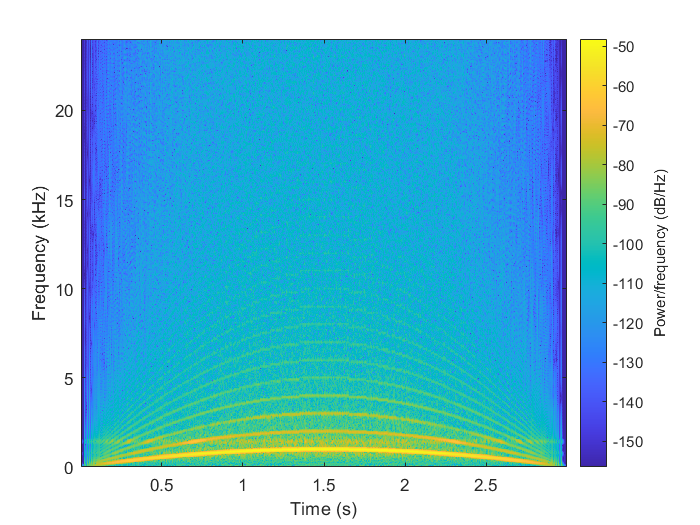
\includegraphics[scale=.60]{./images/plots/NPTResoTanhT60Short.png}
    \caption{Spectrogram of the output from the Noise Pulse Train paired with the Reso + Tanh structure for $T_{60} = $ 2 ms. Note the more clearly defined harmonic structure and comparatively weaker longitudinal mode presence.}
    \label{fig:NPT_RT_T60_Short}
\end{figure}

\begin{figure}[h!]
    \centering
    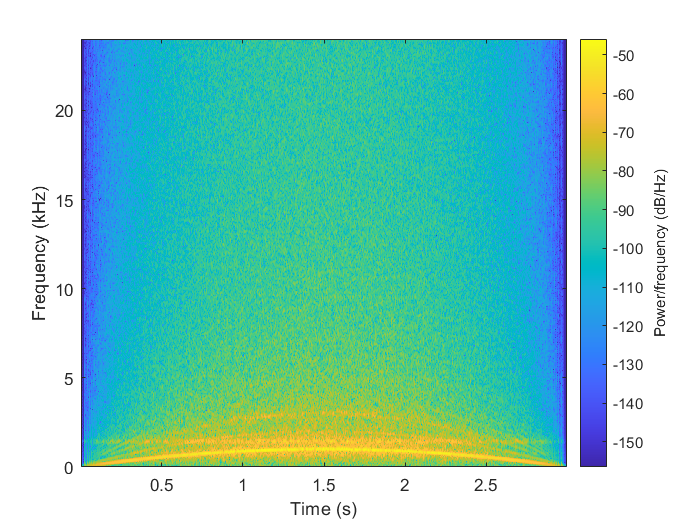
\includegraphics[scale=.60]{./images/plots/NPTResoTanhT60Long.png}
    \caption{Spectrogram of the output from the Noise Pulse Train paired with the Reso + Tanh structure for $T_{60} = $ 20 ms. Note the strong longitudinal mode presence and loss of upper harmonics due to the more noise like structure of the excitation signal.}
    \label{fig:NPT_RT_T60_Long}
\end{figure}

\clearpage

\paragraph{Harmonic Resonator Bank Results:}
Figure~\ref{fig:NPT_HRB_T60_Short} and Fig.~\ref{fig:NPT_HRB_T60_Long} show the spectrograms of the output of the Noise Pulse Train paired with the Harmonic Resonator Bank for the long and short $T_{60}$ values. The Harmonic Resonator Bank was set to only 6 harmonics. The results can be heard in \emph{NPT-HRB-T60-Short.wav} and \emph{NPT-HRB-T60-Long.wav}.

When comparing Fig.~\ref{fig:NPT_HRB_T60_Short} to Fig.~\ref{fig:NPT_RT_T60_Short}, the same strong harmonic structure is present. The use of the Harmonic Resonator Bank puts a strong emphasis on the first six harmonics which can be seen in how Fig.~\ref{fig:NPT_HRB_T60_Short} indicates they are slightly stronger than in Reso + Tanh case. As one would expect, the perceptual result of this is less emphasis on the fundamental frequency which can be heard in the corresponding \emph{.wav} files.

When looking at the results of Fig.~\ref{fig:NPT_HRB_T60_Long}, where the HRB is used with the longer $T_{60}$ value, the most notable feature is the limitation in the number of harmonics corresponding to the configuration of the HRB. The second most prominent aspect is that the energy of the harmonics is spread out over a wider band as compared to the signals generated using the shorter $T_{60}$. This is due to the fact that these harmonics are created by the resonator filters in the HRB itself as the excitation signal is more noise like and lacks a strong harmonic structure. The spread of the energy can be controlled by the width of the resonator. In Fig.~\ref{fig:NPT_HRB_T60_Short}, the resonators act more to accentuate the already existing harmonics in the signal. From a perceptual standpoint, the longer $T_{60}$ here causes a loss in the impulsive aspects of the sound. This in turn causes the output to sound less like it was generated from a periodic set of impacts/collisions and more like the two interacting surfaces smoother.

\begin{figure}[h]
    \centering
    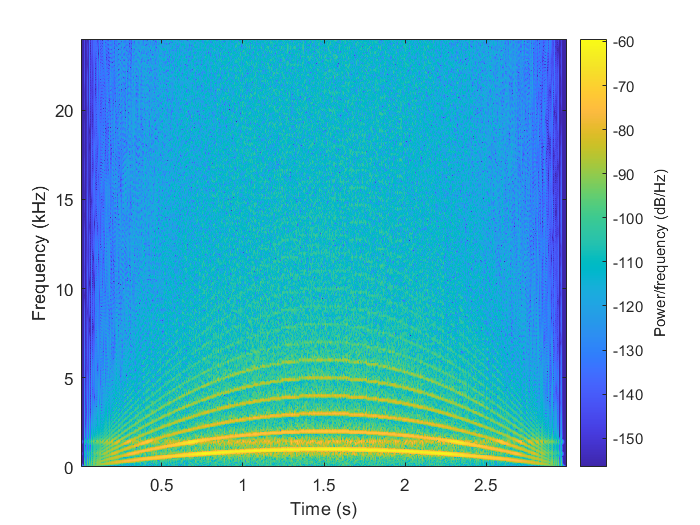
\includegraphics[scale=.65]{./images/plots/NPTHRBT60Short.png}
    \caption{Spectrogram of the output from the Noise Pulse Train paired with the Harmonic Resonator Bank for $T_{60} = $ 2 ms. Compared to the Reso + Tanh approach the harmonics the first 6 harmonics are more emphasized.}
    \label{fig:NPT_HRB_T60_Short}
\end{figure}

\begin{figure}[h]
    \centering
    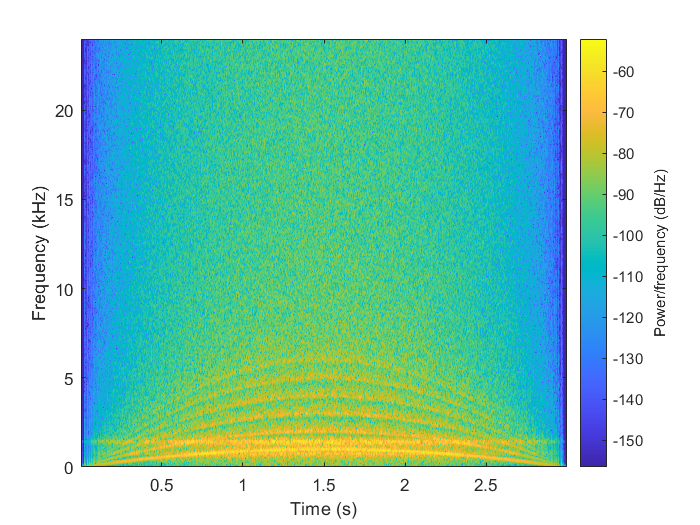
\includegraphics[scale=.65]{./images/plots/NPTHRBT60Long.png}
    \caption{Spectrogram of the output from the Noise Pulse Train paired with the Harmonic Resonator Bank structure for $T_{60} = $ 20 ms. Note that the number of harmonics is limited by the number specified in the HRB and they aren't as energetically concentrated.}
    \label{fig:NPT_HRB_T60_Long}
\end{figure}

% \clearpage

\subsubsection{Noise Burst Generator}
The basis for this structure comes from the guqin model introduced in \citetwo{penttinen_model-based_2006}. As this signal is not inherently harmonic, it does not operate well with the Reso + Tanh approach. Much better results are achieved using the Harmonic Resonator Bank method as the signal itself is much more noise like. However, the Noise Pulse Train provides much better results in the context of the synthesizer given that it creates a harmonic structure and retains an impulsive aspect when $T_{60}$ is tuned properly.

\paragraph{Reso + Tanh Results:}
As mentioned before, it was not expected that this combination of components performed well in the goal of perceptually simulating the strong-to-winding impact sound. Figure~\ref{fig:NBG_RT_T60_Short} and Fig.~\ref{fig:NBG_RT_T60_Long} show spectograms for the results. The sounds can be heard in \emph{NBG-RT-T60-Short.wav} and \emph{NBG-RT-T60-Long.wav}.

These results clearly indicate a lack of harmonic structure. The main spectral components which are present is a band of energy corresponding to the fundamental frequency (which is extracted by the resonator in the Reso + Tanh) as well as a prominent longitudinal mode. Between the two $T_{60}$ parameters, the difference is that the longer $T_{60}$ produces more concentrated energy in the resulting bands due to its inherently more noise like structure.

\clearpage

\begin{figure}[h!]
    \centering
    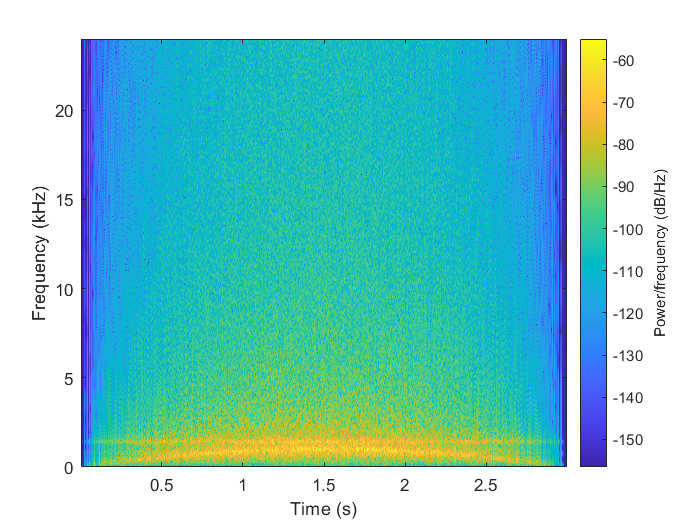
\includegraphics[scale=.60]{./images/plots/NBG-RT-T60-Short.png}
    \caption{Spectrogram of the output from the Noise Burst Generator paired with the Reso + Tanh structure for $T_{60} = $ 2 ms. Only the fundamental and some longitudinal modal effects are present.}
    \label{fig:NBG_RT_T60_Short}
\end{figure}

\begin{figure}[h!]
    \centering
    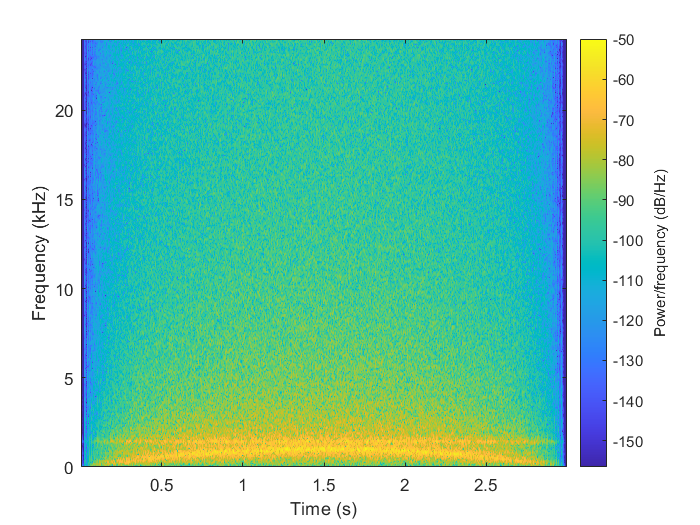
\includegraphics[scale=.60]{./images/plots/NBG-RT-T60-Long.png}
    \caption{Spectrogram of the output from the Noise Burst Generator paired with the Reso + Tanh structure for $T_{60} = $ 20 ms.}
    \label{fig:NBG_RT_T60_Long}
\end{figure}

\clearpage

\paragraph{Harmonic Resonator Bank Results:}
The results of this test are an improvement over the previous, however they do not yield results as good as when the Noise Pulse Train generates the excitation. Figure~\ref{fig:NBG_HRB_T60_Short} and Fig.~\ref{fig:NBG_HRB_T60_Long} illustrate the spectrograms for the short and long $T_{60}$ values respectively. The results can be heard in in \emph{NBG-HRB-T60-Short.wav} and \emph{NBG-HRB-T60-Long.wav}. There is a much clearer harmonic structure as compared to using Reso + Tanh with the Noise Burst Generator. However, the impulsive aspect is not present. This component is necessary to sound like two by two objects are colliding as opposed to just rubbing and creating friction sounds.

\begin{figure}[h!]
    \centering
    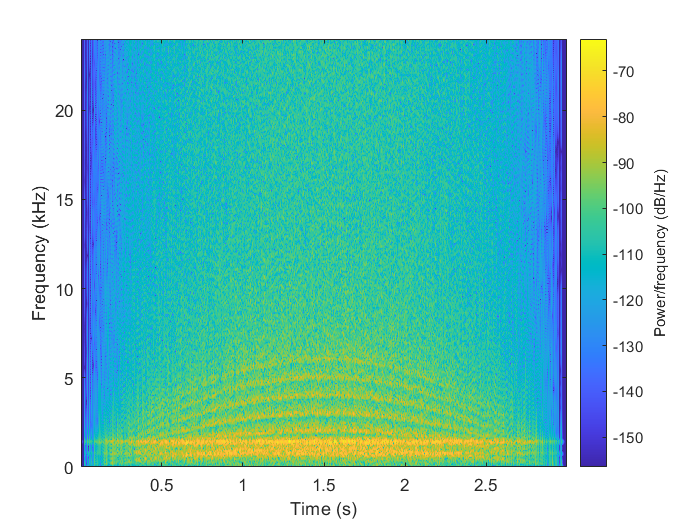
\includegraphics[scale=.65]{./images/plots/NBG-HRB-T60-Short.png}
    \caption{Spectrogram of the output from the Noise Burst Generator paired with the Harmonic Resonator Bank for $T_{60} = $ 2 ms.}
    \label{fig:NBG_HRB_T60_Short}
\end{figure}

\begin{figure}[h!]
    \centering
    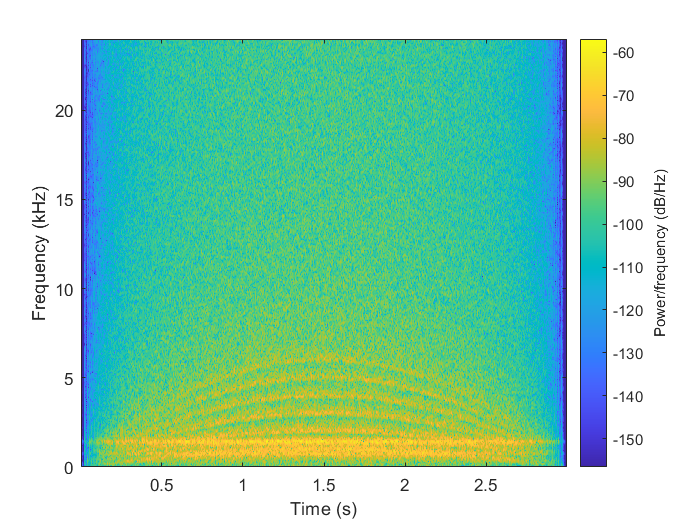
\includegraphics[scale=.65]{./images/plots/NBG-HRB-T60-Long.png}
    \caption{Spectrogram of the output from the Noise Burst Generator paired with the Harmonic Resonator Bank for $T_{60} = $ 20 ms.}
    \label{fig:NBG_HRB_T60_Long}
\end{figure}

% \clearpage

\subsection{Matching the Recordings}
Determining which pair of noise source/harmonic accentuation objects to use, as well as how to tune the parameters of the Wound CSG, was done by comparison using the spectrum from Fig.~\ref{fig:ContactNoiseEBrass} and the corresponding measurements as the baseline. A control curve for $slideSpeed[n]$ was generated to mimic the speed which the slide experienced during the measurements. Subsequently, this was applied to a Wound CSG object tuned to various sets of parameters. The best results are shown in Fig.~\ref{fig:TunedWoundCSG} and can be heard in \emph{Tuned-Wound-CSG.wav}.

\begin{figure}[h]
    \centering
    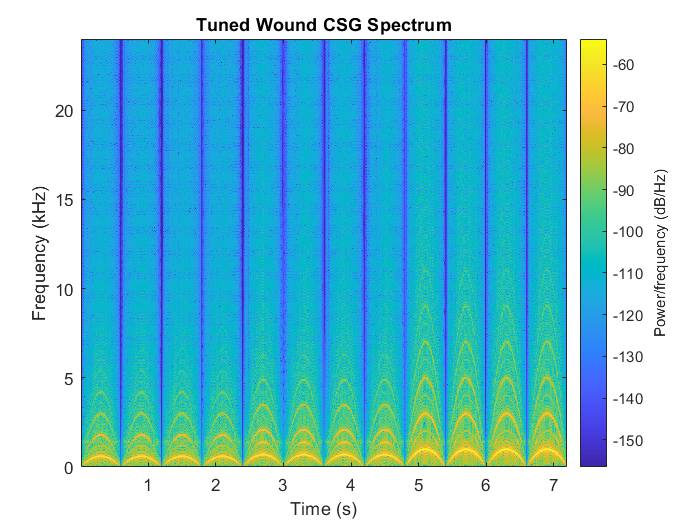
\includegraphics[scale=.65]{./images/plots/TunedWoundCSG.png}
    \caption{Spectrogram of the output from the tuned Wound CSG using the Noise Pulse Train, Reso + Tanh structure, $T_{60} = $ 2 ms and $g_{bal} = .15$.}
    \label{fig:TunedWoundCSG}
\end{figure}

Based on the results of the previous section, it was determined that the best noise source and harmonic accenutator pair is the Noise Pulse Train and Reso + Tanh structure. The harmonics produced using this pair sound subtantially more realistic as compared to the harmonics produced via filtered noise using the HRB. For the tuned $T_{60}$ value, this pair produced a similar number of harmonics to what appears in the last slide event of Fig.~\ref{fig:ContactNoiseEBrass} using a pre-$\tanh()$ gain of 30. The relative-strengths of the odd-order harmonics are increased due to the imperfections in the filtering mechanism by which the fundamental is extracted. This is on avoidable as the resonator which extracts the fundamental has $r = .99$ and cannot be made more frequency selective. These harmonic imbalances could be corrected by adding an HRB structure after the Reso + Tanh to help control the harmonic proportions more easily. However, this would increase the computational complexity of the implementation potentially making it not feasible for a real-time scenario. It is unknown why the slide measurements which occur earlier in the recording, from Fig.~\ref{fig:ContactNoiseEBrass}, do not exhibit the same number of harmonics and overall strength as the corresponding sounds in the synthesized version. There is likely an interaction between the slide and string surfaces which is not described purely by the slide speed or a component which is missing in the model.

In terms of $T_{60}$, experimentation showed that a value of 2 ms in combination with $g_{bal} = .15$ provided the best sounding results while producing a synthesized spectrum which was closest to the measured contact sound characteristics. This $T_{60}$ value provides a balance between being able to generate a harmonic waveform while at the same time providing enough noise like characteristics to stimulate the longitudinal mode filters. Shorter values were unable to properly excite the 4th-order filter, while longer values lacked a harmonic structure enough to produce convincing sounds. The 2 ms value is an order of magnitude lower than the rough estimate from Sec.~\ref{sec:T60Measurement} and two orders lower than the 200 ms listed in Fig.~B6 of \citetwo{puputti_real-time_2010}. This suggests that more research needs to be done to be able to properly measure this quantity and understand its ramifications in the computational model of the sound, whether it be a perceptual approximation or refined to a more accurate physical simulation. 

Given that the only differences between strings for model's implementation are the coefficients for the 4th-order filter and $n_w$, the same tuning values are used across the other strings. This may not be the most physically accurate approach, but given that the CSG sound is an extremely small component of the total synthesized sound any other changes are extremely difficult to perceive in the total output. Verification was done by through the same spectral and perceptual comparison method.

\section{Waveform Initialization}
A variety of different waveforms and pre-processing techniques can be used to initialize the DWG structure. Several of these are described in \citetwo{valimaki_development_1998} and \citetwo{karjalainen_plucked-string_1998} and the topic could span an entire thesis itself. For the purposes of this implementation, white noise and pink noise are provided as options to initialize the DWG and provide different timbral characteristics to the synthesized tone. Pink noise was used in the \citetwo{puputti_real-time_2010} implementation while historically white noise has been used \citetwo{karplus_digital_1983}. In either case, it is necessary to pre-process the waveform to remove any DC bias as this can add unwanted artifacts and build up in the DWG model over time.

\subsection{White vs. Pink Noise}
Each noise type has a different properties regarding its frequency content and spectral makeup. White noise contains equal frequency content across the spectrum, whereas pink noise has a spectrum which has equal energy per octave. Accordingly, pink noise is skewed more towards the lower end of the spectrum while white noise contains more energy at the upper end for a specified sampling rate. 

Perceptually, this different frequency content translates into different timbres of the plucked string. White noise generated signal contains more definition/clarity in the attack as it contains the higher frequencies are necessary to create sharper transitions associated with a faster transient. The pink noise generated sounds have more of a ``warmer" sound due to their stronger low-frequency content and could be considered more natural sounding. Results from the different noise types can be heard in the files \emph{Pluck-pink-noise.wav} and \emph{Pluck-white-noise.wav}.

\subsection{Removing DC Component}
The standard method of removing the DC component from a stored signal is by computing its mean and subtracting this from the waveform. Given that the digital waveguide's length is distributed across three different components (the integer delay line, the interpolation filter and the loop filter) there is a question of where to store the initial waveform inside the computational structures. Through experimentation is was determined that the integer delay line was the best place to achieve this. This is also backed by the theory, as fundamentally it is not possible to generate a digital waveform with an non-integer number of samples. Additionally, the input to the loop filter is subject to the effects of the interpolation filter and as the frequency response characteristics of both filters is dependent on $L[n]$, the process of taking into account their effects when removing the DC bias complicates the matter.

In terms of the actual implementation, a subtle but important distinction to note is the difference between the size of the buffer used to implement the DWG and the length of the DWG itself. Suppose that the data structure for the buffer has been set to have a maximum of 1000 samples but only 250 samples are required for the integer delay line. Only those 250 samples should be considered as those are the only ones which will be used to synthesize the tone. The others will be overwritten as the algorithm computes it output samples due to the feedback connection. Including them in the computations ends up adding an unwanted DC bias as they will influence the computed mean. Contrary to white noise, pink noise is correlated with itself. This property is an additional factor to consider as it results an initialization signal which is not true pink noise if more samples than is necessary are generated.

The files \emph{DC-Bias-Removed.wav} and \emph{DC-Bias-Kept.wav} contain synthesized sounds with and without the DC component removed from the initial waveform. Figure~\ref{fig:DCBiasRemoved} and Fig.~\ref{fig:DCBiasKept} illustrate the spectrogram for each of these two samples respectively. The DC component is most easily seen along the bottom axis during the beginning of the sound in Fig.~\ref{fig:DCBiasKept}.

\begin{figure}[h]
    \centering
    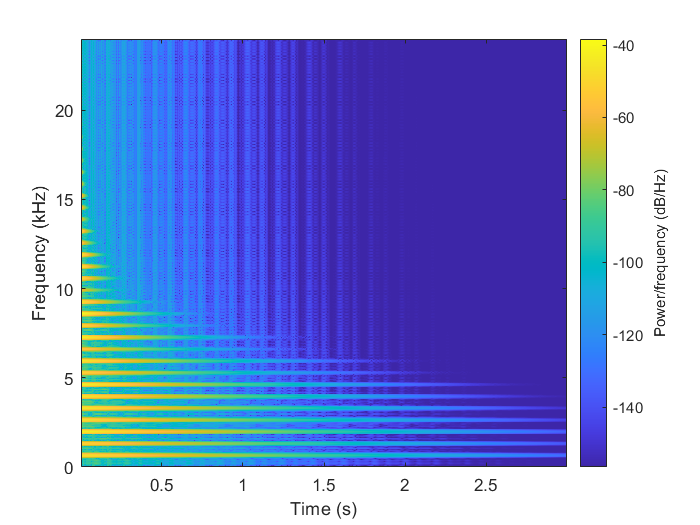
\includegraphics[scale=.65]{./images/plots/DCBiasRemoved.png}
    \caption{Spectrogram of a sound synthesized with the DC bias removed from the initial DWG waveform}
    \label{fig:DCBiasRemoved}
\end{figure}

\begin{figure}[h]
    \centering
    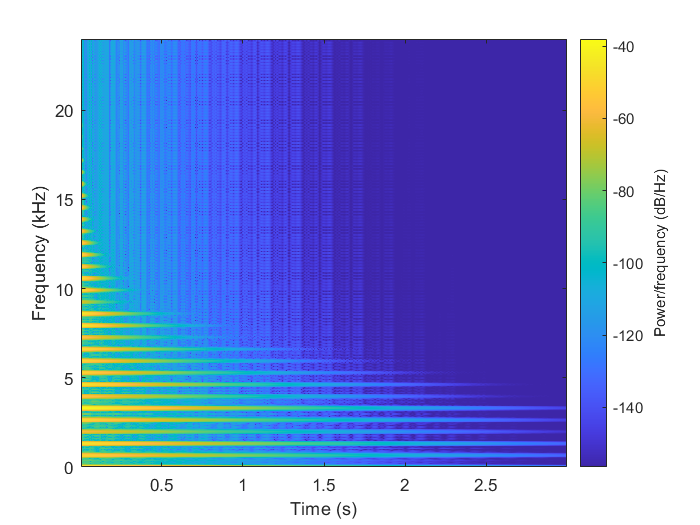
\includegraphics[scale=.65]{./images/plots/DCBiasKept.png}
    \caption{Spectrogram of a sound synthesized with the DC bias kept in the initial DWG waveform. It is most easily identifiable starting in the bottom right corner.}
    \label{fig:DCBiasKept}
\end{figure}

\clearpage

\section{Control Signal Parametrization}
A crucial component in any sound synthesis algorithm is the parametrization and generation of its control signals. This section first introduces the basic algorithms to generate $L[n]$ for different articulations. These results are used to synthesize a musical example of which recordings were also made. The synthesized results are compared to the recorded results in order to understand the differences and limitations of the algorithms described. Musicians have a long history of using equipment outside its intended design. This serves as the creative impetus for the ending discussion of this section where $L[n]$ parameterized to purposefully induce an unstable state in the synthesizer.

\subsection{\emph{L[n]} Generation}
\subsubsection{Algorithm for Arbitrary Slides}
A rudimentary algorithm for generating $L[n]$ was created which results in the synthesized tone following a linear pitch trajectory by taking into account the fact that the ear hears changes in the fundamental frequency logarithmically \citetwo{plack_sense_2018}. Algorithm~\ref{alg:generateLn} describes this in more detail. Based on specified starting and stopping points as well as a duration (in seconds), the algorithm calculates the relative change in string length on a per sample basis based on the logarithmic perception aspects of the ear.

\begin{algorithm}
\caption{Generate logarithmic $L[n]$ from specified end points and duration}
\label{alg:generateLn}
\begin{algorithmic}
\Require $L_{init}$, $L_{end}$, $F_s$, $duration$
\State $frequencyRatio = \frac{L_{init}}{L_{end}}$
\State $numSamples = F_s \times duration$
\State $sampleRatio = frequencyRatio^{\frac{1}{numSamples-1}}$ 
\State $n \gets 0$
\For{$n < numSamples-1$}
    \State $L[n] \gets L_{init} \times sampleRatio^{-n}$
\EndFor
\end{algorithmic}
\end{algorithm}

\subsubsection{Vibrato}
The vibrato signals are generated based on a sinusoidal model which calculates the fret trajectory with the following expression:
\begin{align}
    m_{\text{fret}}[n] &= A\sin(2\pi f_v T_s n) + C\\
    n & = 0, 1, 2, ... , F_s\times  duration - 1\\
\end{align}
where $A$ is the vibrato width in semi-tones (or frets), $f_v$ is the vibrato frequency in Hz, $C$ is the center fret and $duration$ is the length of the vibrato in seconds. $\sin()$ was chosen over $\cos()$ here as this results in $L[n]$ starting at the specified center fret. Once the trajectory of the fret values over time, $m_{\text{fret}}[n]$ is converted to the corresponding relative string length using a slightly rearranged version Eq.~\ref{eq:fretNumber}. The resulting $L[n]$ is used to control the synthesis model.

\subsubsection{Notational Slide-In}
As will be elaborated upon in the next section, this synthesis model was used to generate sounds corresponding to a musical example which is specified in standard musical notation. This example is shown in Fig.~\ref{fig:slideLick}. To generate the \emph{slide-in} articulations, a short segment is generated following Alg.~\ref{alg:generateLn}. For the algorithms parameters, the $duration$ correspond to  a 16th note for the specified tempo, $L_{end}$ is the fret corresponding to the target note, and $L_{init}$ is one fret below $L_{end}$.

\subsection{Comparison to Observed \emph{L[n]}}
The musical example in Fig.~\ref{fig:slideLick} was both synthesized and recorded to facilitate a comparison between the synthesized and observed $L[n]$ signals. For the recorded example, $F_0[n]$ was first estimated using the YIN algorithm \citetwo{de_cheveigne_yin_2002} from which $L[n]$ derived based on Eq.~\ref{eq:F_L}. The results are shown in Fig.~\ref{fig:LnCompare}. Only the segments which the YIN algorithm was extremely confident are are plotted, hence the discontinuities in the graph. It tended to fail during note-onset events. Although a bit of noise exists in the computed signal, more general qualitative comparisons between the two plots can still be made. The sounds being compared can be heard in \emph{SlideLick-High-e-Rec.wav} and \emph{SlideLick-High-e-Synth.wav}.

\begin{figure}[h]
    \centering
    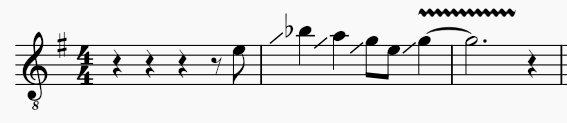
\includegraphics[scale=.75]{./images/pictures/slideLick.png}
    \caption{Slide playing example for the high E string.}
    \label{fig:slideLick}
\end{figure}

\begin{figure}[h]
    \centering
    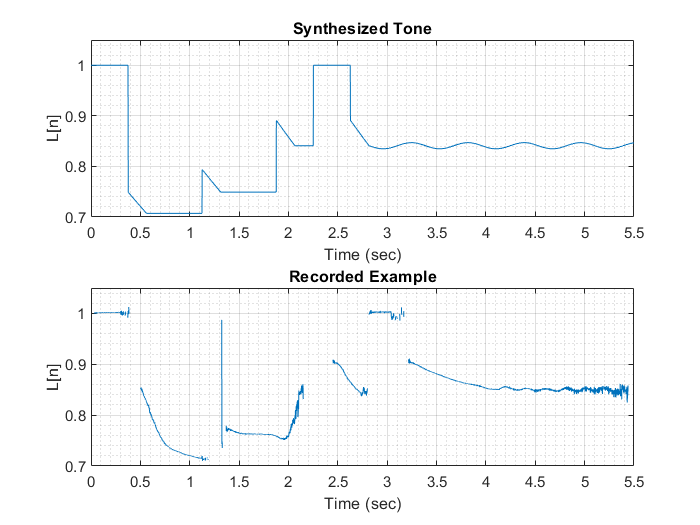
\includegraphics[scale=.65]{./images/plots/L_nComparison.png}
    \caption{$L[n]$ used to synthesize musical example and $L[n]$ computed from a recording of the same sample using the YIN algorithm. Some noise exists due to limitations of the YIN algorithm, however general characteristics can still be compared.}
    \label{fig:LnCompare}
\end{figure}

As can be both seen and heard, the $L[n]$ trajectories which Alg.~\ref{alg:generateLn} produce do not sound quite as nuanced as what is captured in the recorded example. The slopes of the transitions from the recorded example are not constant as they appear in the synthesized tone's transitions. Visually and audibly the recording has more inflection points and the duration of each ``approach" slide is not fixed as in the synthesized example. The second note of the recorded example also includes a slide downwards as it decays. With regards to the vibrato, there is much more of a delay after the initial attack before it is initiated in the recording. Nor is its frequency constant. The synthesized tone transitions much more directly into its vibrato, and maintains the same frequency and amplitude while the note decays (as it was programmed to do). In general, the synthesized example is missing quite a bit of the nuance of the recording. It would be a substantial task in itself to generate mathematical expressions for the recordings subtle details and translate these into an easily parameterized $L[n]$ generation algorithm.

\subsection{Purposeful Instability}
Guitarists, and musicians in general, have a long history of using equipment in a fashion which it was not originally designed to be done. Distortion is an example of this. From an engineering standpoint, it is generally taught that distortion not desirable and is often defined as ``an un-wanted component in the output signal". Since its initial ``discovery", distortion has become an integral part of the tone of an electric guitar to the point where amplifiers are designed to purposely create it in a musical way. The following experiment was done in a similar vein of where the synthesis model is pushed into an unstable (and initially undesirable) state to see what the output is produced.

As noted in the discussion in Sec.~\ref{sec:MinL}, it is possible to adjust $L[n]$ in such a fashion that it the loop filter has positive gain at certain frequencies. Given its placement in a feedback loop, this could put the synthesis model in an unstable state. In order to ensure the system is unstable, another condition needs to be met. It would be necessary for the attenuation provided by the interpolation filter to be less than the amplification of the loop filter so the net loop gain would be positive. The integer delay component has unity gain so it does not need to be considered here. A Lagrange interpolation filter will have unity gain when it does not need to provide any interpolation on the waveform in the DWG. This occurs when the fractional component of the total digital waveguide length can be achieved via the via phase delay of the loop filter.

The relative string length can be expressed as:

\begin{equation}
    L = \frac{OpenString_{F_0}}{F_s} \times DWGLength    
\end{equation}
Given an open-string fundamental frequency and sampling rate, only the appropriate digital waveguide length needs to be selected. For the D-string running at 48kHz and using an approximation of .25 for the loop filter's phase delay, the following calculation produces an unstable system without going beyond the 24th fret (keeping it in the range of many electric guitars):

\begin{equation}
\label{eq:LUnstable}
    L = \frac{146.83}{48,000} \times 82.25 \approx .2516
\end{equation}

The results of this system are illustrated in Fig.~\ref{fig:UnstableLoop}. This clearly shows how the upper frequencies are amplified over time as the system maintains an unstable state. Based on the magnitude responses shown in Fig.~\ref{fig:UnstableLoopString4}, this is expected behavior. Two output files exist for this example: \emph{UnstableOutput-scaled.wav} and \emph{UnstableOutput-clipped.wav}. In order to be able to save the output without clipping, it was necessary to scale/normalize it first. However, the scaling was so drastic due to the extremes in signal values that the output doesn't contain much useful information. In a real-time system, the instability would likely manifest as clipping so a file was produced where the clipping was allowed to occur. Ultimately the musicality of this sound is subject to the creative desires of the composer utilizing it, however the harsher and more chaotic sounds of the clipped example could find use in electronic or industrial music genres.

\begin{figure}[h]
    \centering
    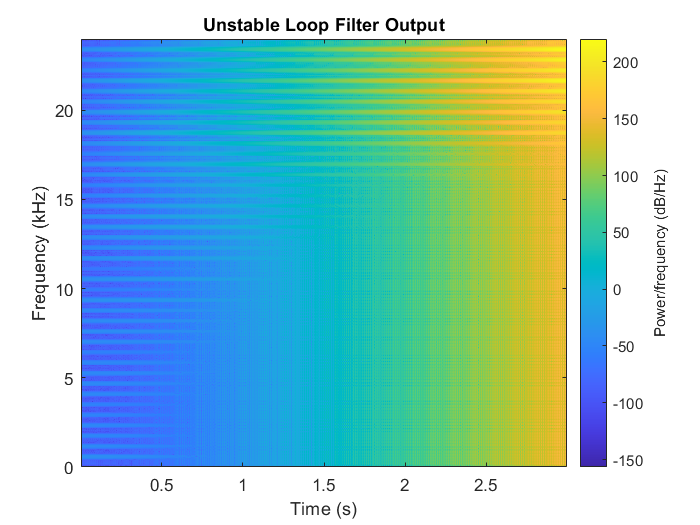
\includegraphics[scale=.65]{./images/plots/UnstableLoopFilter.png}
    \caption{Spectrogram of the sound synthesized after the model has been put in an unstable state using the $L$ value from Eq.~\ref{eq:LUnstable}}
    \label{fig:UnstableLoop}
\end{figure}

\end{document}